% questions.tex —— 2004 年·普通高等学校招生考试·重庆卷·理科 · 题目内容片段（无答案）
% 由 tools/generate_projects.py 依来源总账自 2004/2004_数学真题_重庆理科_试题.md 生成，勿手改（改源 MD 后重跑）

\gkpart{一、选择题：本大题共 12 小题，每小题 5 分，共 60 分．在每小题给出的四个选项中，只有一项是符合题目要求的．}

\begin{question}
\gkti{1}函数 $y = \sqrt{\log_{\frac{1}{2}}(3x - 2)}$ 的定义域是\mbox{（　　）}

\begin{gkopts}(2)
\task A．$[1, +\infty)$
\task B．$\left(\dfrac{2}{3}, +\infty\right)$
\task C．$\left[\dfrac{2}{3}, 1\right]$
\task D．$\left(\dfrac{2}{3}, 1\right]$
\end{gkopts}

\end{question}
\begin{question}
\gkti{2}设复数 $Z = 1 + \sqrt{2}\mathrm{i}$，则 $Z^2 - 2Z =$\mbox{（　　）}

\begin{gkopts}(4)
\task A．$-3$
\task B．$3$
\task C．$-3\mathrm{i}$
\task D．$3\mathrm{i}$
\end{gkopts}

\end{question}
\begin{question}
\gkti{3}圆 $x^2 + y^2 - 2x + 4y + 3 = 0$ 的圆心到直线 $x - y = 1$ 的距离为\mbox{（　　）}

\begin{gkopts}(2)
\task A．$2$
\task B．$\dfrac{\sqrt{2}}{2}$
\task C．$1$
\task D．$\sqrt{2}$
\end{gkopts}

\end{question}
\begin{question}
\gkti{4}不等式 $x + \dfrac{2}{x + 1} > 2$ 的解集是\mbox{（　　）}

\begin{gkopts}(2)
\task A．$(-1, 0) \cup (1, +\infty)$
\task B．$(-\infty, -1) \cup (0, 1)$
\task C．$(-1, 0) \cup (0, 1)$
\task D．$(-\infty, -1) \cup (1, +\infty)$
\end{gkopts}

\end{question}
\begin{question}
\gkti{5}$\sin 163^\circ \sin 223^\circ + \sin 253^\circ \sin 313^\circ =$\mbox{（　　）}

\begin{gkopts}(2)
\task A．$-\dfrac{1}{2}$
\task B．$\dfrac{1}{2}$
\task C．$-\dfrac{\sqrt{3}}{2}$
\task D．$\dfrac{\sqrt{3}}{2}$
\end{gkopts}

\end{question}
\begin{question}
\gkti{6}若向量 $\vec{a}$ 与 $\vec{b}$ 的夹角为 $60^\circ$，$|\vec{b}| = 4$，$(\vec{a} + 2\vec{b}) \cdot (\vec{a} - 3\vec{b}) = -72$，则向量 $\vec{a}$ 的模为\mbox{（　　）}

\begin{gkopts}(4)
\task A．$2$
\task B．$4$
\task C．$6$
\task D．$12$
\end{gkopts}

\end{question}
\begin{question}
\gkti{7}一元二次方程 $ax^2 + 2x + 1 = 0$ ($a \neq 0$) 有一个正根和一个负根的充分不必要条件是\mbox{（　　）}

\begin{gkopts}(4)
\task A．$a < 0$
\task B．$a > 0$
\task C．$a < -1$
\task D．$a > 1$
\end{gkopts}

\end{question}
\begin{question}
\gkti{8}设 $P$ 是 $60^\circ$ 的二面角 $\alpha - l - \beta$ 内一点，$PA \perp$ 平面 $\alpha$，$PB \perp$ 平面 $\beta$，$A, B$ 为垂足，$PA = 4$，$PB = 2$，则 $AB$ 的长为\mbox{（　　）}

\begin{gkopts}(4)
\task A．$2\sqrt{3}$
\task B．$2\sqrt{5}$
\task C．$2\sqrt{7}$
\task D．$4\sqrt{2}$
\end{gkopts}

\end{question}
\begin{question}
\gkti{9}若数列 $\{a_n\}$ 是等差数列，首项 $a_1 > 0$，$a_{2003} + a_{2004} > 0$，$a_{2003} \cdot a_{2004} < 0$，则使前 $n$ 项和 $S_n > 0$ 成立的最大自然数 $n$ 是\mbox{（　　）}

\begin{gkopts}(4)
\task A．$4005$
\task B．$4006$
\task C．$4007$
\task D．$4008$
\end{gkopts}

\end{question}
\begin{question}
\gkti{10}已知双曲线 $\dfrac{x^2}{a^2} - \dfrac{y^2}{b^2} = 1$ ($a > 0, b > 0$) 的左、右焦点分别为 $F_1, F_2$，点 $P$ 在双曲线的右支上，且 $|PF_1| = 4|PF_2|$，则此双曲线的离心率 $e$ 的最大值为\mbox{（　　）}

\begin{gkopts}(4)
\task A．$\dfrac{4}{3}$
\task B．$\dfrac{5}{3}$
\task C．$2$
\task D．$\dfrac{7}{3}$
\end{gkopts}

\end{question}
\begin{question}
\gkti{11}某校高三年级举行一次演讲赛共有 $10$ 位同学参赛，其中一班有 $3$ 位，二班有 $2$ 位，其它班有 $5$ 位，若采用抽签的方式确定他们的演讲顺序，则一班有 $3$ 位同学恰好被排在一起（指演讲序号相连），而二班的 $2$ 位同学没有被排在一起的概率为\mbox{（　　）}

\begin{gkopts}(4)
\task A．$\dfrac{1}{10}$
\task B．$\dfrac{1}{20}$
\task C．$\dfrac{1}{40}$
\task D．$\dfrac{1}{120}$
\end{gkopts}

\Needspace{0.4\textheight}
\end{question}
\begin{question}
\gkti{12}若三棱锥 $A - BCD$ 的侧面 $ABC$ 内一动点 $P$ 到底面 $BCD$ 的距离与到棱 $AB$ 的距离相等，则动点 $P$ 的轨迹与 $\triangle ABC$ 组成图形可能是\mbox{（　　）}
\nopagebreak[4]
\begin{center}% Source-faithful schematic draft: 2004 Chongqing Science Q12, PDF p.1 (printed p.160).
% Source ID: src-f4f7a5339a68a3cbcf5ef54e4d3736a907b6de9c04c1ef9f3f8b8f7b718d56c4
% Source SHA-256: ef3530a818ad893a36345110d6aa9588de3b793de24c4d6f80333cffa317e429
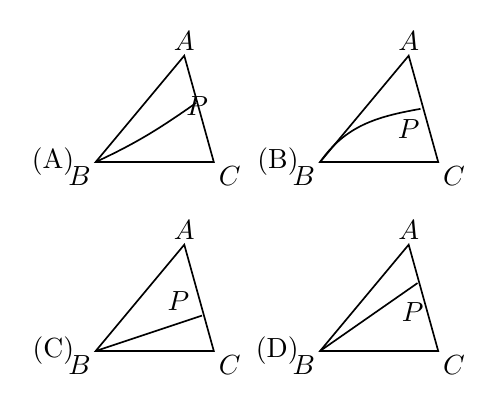
\begin{tikzpicture}[line width=0.6pt, scale=0.75, every node/.style={inner sep=1.5pt}, baseline=(current bounding box.center)]
  % Subfigure (A)
  \begin{scope}[shift={(0, 3.2)}]
    \coordinate (B) at (0, 0);
    \coordinate (C) at (2.0, 0);
    \coordinate (A) at (1.5, 1.8);
    \draw (B) -- (C) -- (A) -- cycle;
    \draw (B) to[out=25, in=215] (1.7, 1.0);
    \node[above] at (A) {$A$};
    \node[below left] at (B) {$B$};
    \node[below right] at (C) {$C$};
    \node[right] at (1.45, 0.95) {$P$};
    \node[left=6pt] at (B) {(A)};
  \end{scope}

  % Subfigure (B)
  \begin{scope}[shift={(3.8, 3.2)}]
    \coordinate (B) at (0, 0);
    \coordinate (C) at (2.0, 0);
    \coordinate (A) at (1.5, 1.8);
    \draw (B) -- (C) -- (A) -- cycle;
    \draw (B) to[out=55, in=190] (1.7, 0.9);
    \node[above] at (A) {$A$};
    \node[below left] at (B) {$B$};
    \node[below right] at (C) {$C$};
    \node[below] at (1.5, 0.8) {$P$};
    \node[left=6pt] at (B) {(B)};
  \end{scope}

  % Subfigure (C)
  \begin{scope}[shift={(0, 0)}]
    \coordinate (B) at (0, 0);
    \coordinate (C) at (2.0, 0);
    \coordinate (A) at (1.5, 1.8);
    \draw (B) -- (C) -- (A) -- cycle;
    \draw (B) -- (1.8, 0.6);
    \node[above] at (A) {$A$};
    \node[below left] at (B) {$B$};
    \node[below right] at (C) {$C$};
    \node[above] at (1.4, 0.6) {$P$};
    \node[left=6pt] at (B) {(C)};
  \end{scope}

  % Subfigure (D)
  \begin{scope}[shift={(3.8, 0)}]
    \coordinate (B) at (0, 0);
    \coordinate (C) at (2.0, 0);
    \coordinate (A) at (1.5, 1.8);
    \draw (B) -- (C) -- (A) -- cycle;
    \draw (B) -- (1.65, 1.15);
    \node[above] at (A) {$A$};
    \node[below left] at (B) {$B$};
    \node[below right] at (C) {$C$};
    \node[below right] at (1.3, 0.9) {$P$};
    \node[left=6pt] at (B) {(D)};
  \end{scope}
\end{tikzpicture}
\end{center}
\nopagebreak[4]
\begin{gkopts}(4)
\task A．见图 (A)
\task B．见图 (B)
\task C．见图 (C)
\task D．见图 (D)
\end{gkopts}

\end{question}
\gkpart{二、填空题：本大题共 4 小题，每小题 4 分，共 16 分．把答案填在横线上．}

\begin{question}
\gkti{13}若在 $(1 + ax)^5$ 的展开式中 $x^3$ 的系数为 $-80$，则 $a =$ \gkblank{}．

\end{question}
\begin{question}
\gkti{14}曲线 $y = 2 - \dfrac{1}{2}x^2$ 与 $y = \dfrac{1}{4}x^3 - 2$ 在交点处切线的夹角是 \gkblank{}．（用弧度数作答）

\Needspace{0.4\textheight}
\end{question}
\begin{question}
\gkti{15}如图 $P_1$ 是一块半径为 $1$ 的半圆形纸板，在 $P_1$ 的左下端剪去一个半径为 $\dfrac{1}{2}$ 的半圆后得到图形 $P_2$，然后依次剪去一个更小半圆（其直径为前一个被剪掉半圆的半径）得图形 $P_3$、$P_4$、$\cdots$、$P_n$、$\cdots$，记纸板 $P_n$ 的面积为 $S_n$，则 $\lim_{n \to \infty} S_n =$ \gkblank{}．
\nopagebreak[4]
\begin{center}% Source-faithful schematic draft: 2004 Chongqing Science Q15, PDF p.1 (printed p.160).
% Source ID: src-f4f7a5339a68a3cbcf5ef54e4d3736a907b6de9c04c1ef9f3f8b8f7b718d56c4
% Source SHA-256: ef3530a818ad893a36345110d6aa9588de3b793de24c4d6f80333cffa317e429
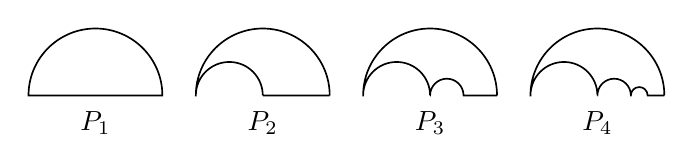
\begin{tikzpicture}[line width=0.6pt, scale=0.85, every node/.style={inner sep=1.5pt}, baseline=(current bounding box.center)]
  % P1: Complete semicircle of radius 1
  \begin{scope}[shift={(0, 0)}]
    \draw (0, 0) -- (2, 0) arc[start angle=0, end angle=180, radius=1] -- cycle;
    \node[below=4pt] at (1, 0) {$P_1$};
  \end{scope}

  % P2: Semicircle with a smaller semicircle of radius 1/2 cut from left
  \begin{scope}[shift={(2.5, 0)}]
    \draw (1, 0) arc[start angle=0, end angle=180, radius=0.5] -- (0, 0) arc[start angle=180, end angle=0, radius=1] -- (2, 0) -- (1, 0);
    \node[below=4pt] at (1, 0) {$P_2$};
  \end{scope}

  % P3: Semicircle with second cut of radius 1/4
  \begin{scope}[shift={(5.0, 0)}]
    \draw (1, 0) arc[start angle=0, end angle=180, radius=0.5] -- (0, 0) arc[start angle=180, end angle=0, radius=1] -- (2, 0) -- (1.5, 0) arc[start angle=0, end angle=180, radius=0.25] -- (1, 0);
    \node[below=4pt] at (1, 0) {$P_3$};
  \end{scope}

  % P4: Semicircle with third cut of radius 1/8
  \begin{scope}[shift={(7.5, 0)}]
    \draw (1, 0) arc[start angle=0, end angle=180, radius=0.5] -- (0, 0) arc[start angle=180, end angle=0, radius=1] -- (2, 0) -- (1.75, 0) arc[start angle=0, end angle=180, radius=0.125] -- (1.5, 0) arc[start angle=0, end angle=180, radius=0.25] -- (1, 0);
    \node[below=4pt] at (1, 0) {$P_4$};
  \end{scope}
\end{tikzpicture}
\end{center}
\nopagebreak[4]
\end{question}
\begin{question}
\gkti{16}对任意实数 $k$，直线 $y = kx + b$ 与椭圆 $\begin{cases} x = \sqrt{3} + 2\cos\theta, \\ y = 1 + 4\sin\theta \end{cases}$ ($0 \leqslant \theta \leqslant 2\pi$) 恰有一个公共点，则 $b$ 取值范围是 \gkblank{}．

\end{question}
\gkpart{三、解答题：本大题共 6 小题，共 74 分．解答应写出文字说明、证明过程或演算步骤．}

\begin{question}
\gkti{17}求函数 $y = \sin^4 x + 2\sqrt{3} \sin x \cos x - \cos^4 x$ 的最小正周期和最小值；并写出该函数在 $[0, \pi]$ 上的单调递增区间．

\end{question}
\begin{question}
\gkti{18}设一汽车在前进途中要经过 $4$ 个路口，汽车在每个路口遇到绿灯的概率为 $\dfrac{3}{4}$，遇到红灯（禁止通行）的概率为 $\dfrac{1}{4}$．假定汽车只在遇到红灯或到达目的地才停止前进，$\xi$ 表示停车时已经通过的路口数，求：

(1) $\xi$ 的概率分布列及期望 $E\xi$；

(2) 停车时最多已通过 $3$ 个路口的概率．

\Needspace{0.4\textheight}
\end{question}
\begin{question}
\gkti{19}如图，四棱锥 $P - ABCD$ 的底面是正方形，$PA \perp$ 底面 $ABCD$，$AE \perp PD$，$EF \parallel CD$，$AM = EF$．
\nopagebreak[4]
\begin{center}% Source-faithful schematic draft: 2004 Chongqing Science Q19, PDF p.1 (printed p.160).
% Source ID: src-f4f7a5339a68a3cbcf5ef54e4d3736a907b6de9c04c1ef9f3f8b8f7b718d56c4
% Source SHA-256: ef3530a818ad893a36345110d6aa9588de3b793de24c4d6f80333cffa317e429
\begin{tikzpicture}[line width=0.6pt, scale=1.1, every node/.style={inner sep=1.5pt}, baseline=(current bounding box.center)]
  % Coordinates of pyramid P-ABCD with square base ABCD
  % A is in the back, PA is perpendicular to base ABCD
  \coordinate (A) at (0, 0);
  \coordinate (D) at (2.4, 0.0);
  \coordinate (B) at (-0.8, -1.1);
  \coordinate (C) at ($(B)+(D)-(A)$); % (1.6, -1.1)
  \coordinate (P) at (0, 3.8);

  % Points E, F, M
  \coordinate (E) at ($(P)!0.62!(D)$);
  \coordinate (F) at ($(P)!0.62!(C)$);
  \coordinate (M) at ($(A)!0.62!(B)$);

  % Dashed internal edges
  \draw[dashed, line width=0.5pt] (P) -- (A);
  \draw[dashed, line width=0.5pt] (A) -- (B);
  \draw[dashed, line width=0.5pt] (A) -- (D);
  \draw[dashed, line width=0.5pt] (A) -- (C);
  \draw[dashed, line width=0.5pt] (A) -- (E);
  \draw[dashed, line width=0.5pt] (A) -- (F);
  \draw[dashed, line width=0.5pt] (M) -- (F);

  % Solid exterior edges
  \draw (P) -- (B);
  \draw (P) -- (C);
  \draw (P) -- (D);
  \draw (B) -- (C);
  \draw (C) -- (D);
  \draw (E) -- (F);

  % Vertex labels faithful to original layout
  \node[above] at (P) {$P$};
  \node[above left] at (A) {$A$};
  \node[below left] at (B) {$B$};
  \node[below right] at (C) {$C$};
  \node[right] at (D) {$D$};
  \node[above right] at (E) {$E$};
  \node[below right] at (F) {$F$};
  \node[left] at (M) {$M$};
\end{tikzpicture}
\end{center}
\nopagebreak[4]
(1) 证明：$MF$ 是异面直线 $AB$ 与 $PC$ 的公垂线；

(2) 若 $PA = 3AB$，求直线 $AC$ 与平面 $EAM$ 所成角的正弦值．

\end{question}
\begin{question}
\gkti{20}设函数 $f(x) = x(x - 1)(x - a)$ ($a > 1$)．

(1) 求导数 $f'(x)$，并证明 $f(x)$ 有两个不同的极值点 $x_1, x_2$；

(2) 若不等式 $f(x_1) + f(x_2) \leqslant 0$ 成立，求 $a$ 的取值范围．

\end{question}
\begin{question}
\gkti{21}设 $p > 0$ 是一常数，过点 $Q(2p, 0)$ 的直线与抛物线 $y^2 = 2px$ 交于相异两点 $A\text{、}B$，以线段 $AB$ 为直径作圆 $H$（$H$ 为圆心）．试证抛物线顶点在圆 $H$ 的圆周上；并求圆 $H$ 的面积最小时直线 $AB$ 的方程．

\end{question}
\begin{question}
\gkti{22}设数列 $\{a_n\}$ 满足 $a_1 = 2$，$a_{n+1} = a_n + \dfrac{1}{a_n}$ ($n = 1, 2, 3, \cdots$)．

(1) 证明 $a_n > \sqrt{2n + 1}$ 对一切正整数 $n$ 成立；

(2) 令 $b_n = \dfrac{a_n}{\sqrt{n}}$ ($n = 1, 2, 3, \cdots$)，判断 $b_n$ 与 $b_{n+1}$ 的大小，并说明理由．

\end{question}